%        File: report.tex
%     Created: Sat Nov 03 06:00 PM 2018 E
% Last Change: Sat Nov 03 06:00 PM 2018 E
%
\documentclass[a4paper]{article}
\usepackage{amsmath}
\usepackage{graphicx}
\usepackage{hyperref}
\usepackage[noabbrev,capitalise]{cleveref}
\usepackage{natbib}

\newcommand{\var}{\text{Var}}

\begin{document}

\title{Baby Name Popularity}
\author{
Francisco Rivera \\ \texttt{frivera@college.harvard.edu}
\and
Mark Chamberlain \\ \texttt{mark\_chamberlain@college.harvard.edu}}

\maketitle

\begin{abstract}

The U.S. Census publishes the number of babies born to each first name each year
at the country-level. It has previously \citep{hahn2003drift} been suggested
these trends could be explained by a simple imitation model where parents copy
baby names from the previous year at random. However, we find these trends
exhibit dramatic up- and down-swings unexplainable by this simple model. We
propose a segmented-population model to explain the observed data. Our model
succeeds in fitting the data and is very suggestive of an agent-based generative
process, but suffers from numerical instabilities in parameter choices and 

\end{abstract}

\section{The Data}

Our data comes from the U.S.
Census.\footnote{\url{https://catalog.data.gov/dataset/baby-names-from-social-security-card-applications-national-level-data}}
The dataset allows us to observe the number of births in the country each year
by first name and gender with the exception of names for which there were fewer
than five births.

The data requires little processing, but because our aim is to model changes in
popularity rather than population growth, we normalize each data entry as a
percentage of the total number of births that year. To provide a sense of what
some typical trends look like, we plot the popularity of five random
popular\footnote{Defined as exceeding 0.5\% of all births on any year.} names in
\cref{fig:fivenames}.

\begin{figure}[h]
\centering
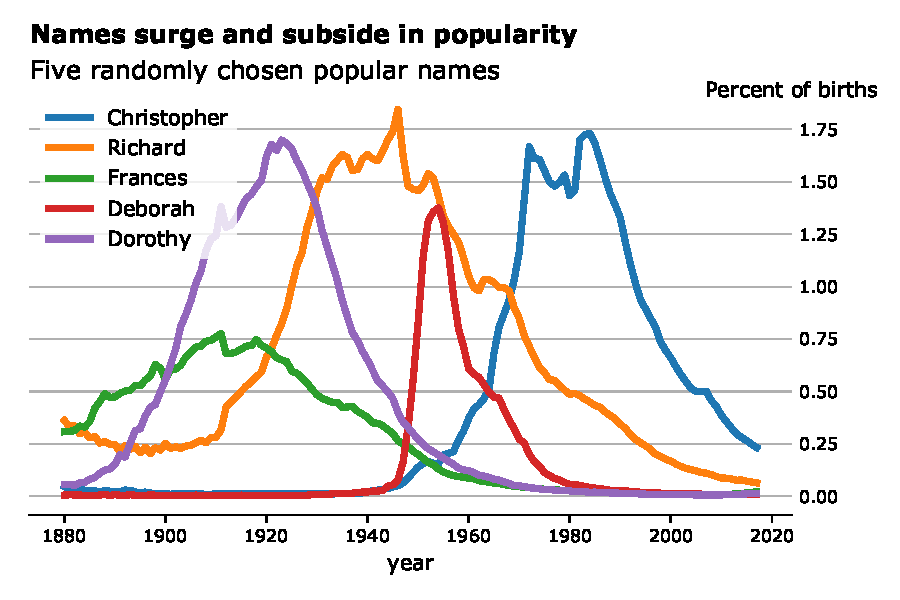
\includegraphics[width=.9\textwidth]{figs/five-rand-names}
\caption{Popularity evolution of five random names}
\label{fig:fivenames}
\end{figure}

On the basis of inspecting many realizations of \cref{fig:fivenames}, for which
the depicted trends are representative, we can take away some stylized facts,

\begin{itemize}
\item The popularity of a name in many cases follows a exponential-like growth
from obscurity, a peak, and then a decay back to obscurity.
\item There appears to be a practical upper-bound to how high the peak gets, but
many (unpopular) names never get close to that upper-bound.
\item As ``Deborah'' shows, the down-swing need not be as fast as the up-swing.
\end{itemize}

\section{An Imitation Model}

We follow the gist of \cite{hahn2003drift}. At its core, the model is
straightforward: we assume that every time period (i.e. each year) every baby is
born by choosing a random baby from the previous time period and copying that
name. \cite{hahn2003drift} highlights the main strengths of this model which
are two-fold,

\begin{itemize}
\item It is extremely parsimonious. There is some nuance surrounding
initialization, but they find that when initializing to individually different
names in epoch 1, the model converges after only a couple hundred time periods.
Beyond that, the model has no parameters to fit and its assumption of
consecutive time-period copying is sensible.

\item The cross-sectional distribution of baby-name popularity matches the
power-law predicted by this imitation model. That is, in any given year, the
distribution of the popularity of different names is consistent with the
dynamics of this model.
\end{itemize}

We accept these strengths at face value, but question whether this model is
sufficient to model the inter-temporal aspect as well. To test this, we
introduce some notation. For the $i^\text{th}$ name let $p_t^{(i)}$ represent
the proportion of the number of births in year $t$ to name $i$. Our key model
assumption is that,
\[ p_{t+1}^{(i)} \sim \frac{1}{N_{t+1}} \cdot \text{Binom}(N_{t+1}, p_t^{(i)}).\]
This formula also explains why we are not concerned with the initial conditions
of the model: conditional on the previous time period's distribution, the model
dictates a probability distribution over the following period. 

\begin{figure}[h]
\centering
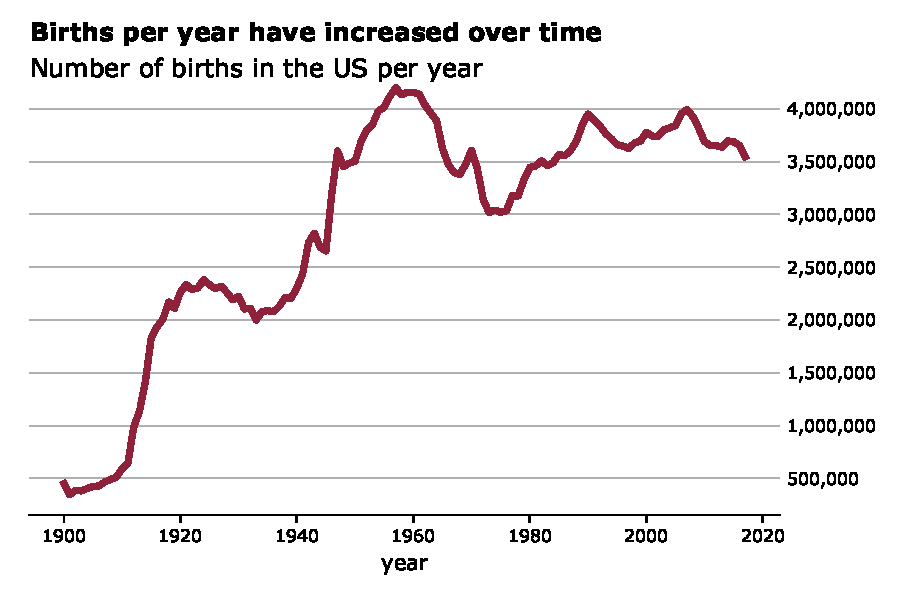
\includegraphics[width=.9\textwidth]{figs/births-per-year.pdf}
\caption{Births per year}
\label{fig:birthsyear}
\end{figure}

In particular, the only parameter in this equation is the number of births which
is easily observable. We plot the number of births per years in
\cref{fig:birthsyear}. This graphs shows us that while births have generally
been increasing over the course of the 20th century, the number of births has
remained approximately the same order of magnitude, and for the latter part of
the century can be reasonably approximated as $N_t \approx 3.5 \times 10^6$.

This allows us to calculate
\[ \var(p_{t+1}^{(i)} \mid p_t^{(i)}) =
\frac{p_t^{(i)}(1-p_t^{(i)})}{N_{t+1}}\]
In particular, if $p$ is moderately large to say that the distribution of
$p_{t+1}^{(i)} \mid p_t^{(i)}$ is approximately distributed as,
\[ \mathcal{N}\left( p_t^{(i)}, \frac{p_t^{(i)}(1-p_t^{(i)})}{N_{t+1}} \right)\]
For small values of $p_t$, $1-p_t^{(i)} \approx 1$ and our standard deviation
will be approximately,
\[ \frac{\sqrt{p_t^{(i)}}}{\sqrt{N_{t+1}}} \approx \frac{\sqrt{p_t^{(i)}}}{10^3}.\]

For $p_t^{(i)} = 1\%$ this means that the year-on-year standard deviation
becomes $10^{-4}$. If $p_t^{(i)} = 0.01\% = 10^{-4}$ the year-on-year standard
deviation becomes $10^{-5}$. And if $p_t = 10^{-6}$ the year-on-year standard
deviation will be approximately $10^{-6}$. This illustrates an important
consequence of this model: the because the standard deviation scales as
approximately the square root of the popularity of the names (for small enough
popularities, where the $1-p_t^{(i)}$ is approximately 1), we have that the
standard deviation as a multiple of the proportion is bigger for smaller
probabilities.

Put more concretely, we are unsurprised if a very unpopular name doubles in
popularity from one year to another, but are quite surprised if this happens for
a more popular name. However, does this prediction survive the data? 

\cref{fig:imitation-pred} illustrates a resounding no. In it, we depict 100
randomly generated paths from the imitation model superimposed on a starting
condition for the popularity of the name ``Amanda,'' as well as the actual
realized trend. We see that according to this model, the boom in popularity of
the name ``Amanda'' from 0.5\% of the popularity to 2.5\% of the yearly baby
population would be near-impossible. This is not a cherry-picked example: these
swings in popularity constantly appear across the trends of different names.

\begin{figure}[h]
\centering
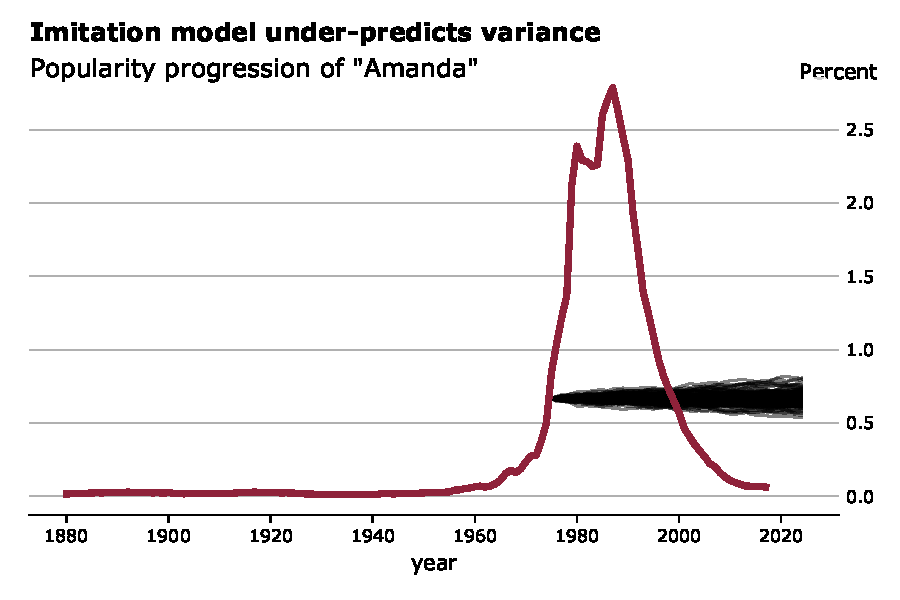
\includegraphics[width=.9\textwidth]{figs/imitation-model}
\caption{Imitation model predictions}
\label{fig:imitation-pred}
\end{figure}

\cref{fig:imitation-pred} runs the model using the precise yearly births and
generating binomial random variables. What we get looks an awfully lot like
Brownian motion, though, which we can explain by our previous observation. We
had previously noted that the binomial tends toward a Normal by the Central
Limit Theorem, and when
\[ \sqrt{\var(p_{t+1}^{(i)} \mid p_t^{(i)})} \ll p_t \]
we have that,
\[ p_{t+1} \approx p_t \implies \var(p_{t+1}^{(i)} \mid p_t^{(i)}) \approx \var(p_{t+2}^{(i)} \mid
p_{t+1}^{(i)}) \]
giving us an approximation to the model prediction for uncertainty $k$ years
into the future as,
\[ \var(p_{t+k}^{(i)} \mid p_t^{(i)}) \approx k \cdot
\frac{p_t^{(i)}(1-p_t^{(i)})}{N_{t+1}}.\]
However, we face the fact that our trends look distinctly unlike Brownian
motion, and we must consider a different model to explain the shape of these
trends.

\section{Segmenting the population}

Another way to view the shortcomings of the imitation model or a model like it
is that the evolution of name popularity appears to behave differently on the
up-swing than the down-swing. This became starkly inconsistent with the
imitation model in the amount of variance we see from year-to-year in name
popularity, but even if the variance matched, we consistently see a boom
followed by a bust in name popularity, which remains unexplainable by this
model.

This suggests that there is something different in the adoption of a name at
different points in the stylized life-cycle of popularity. One way to model this
is by segmenting the population, akin to the work on fads done in
\cite{bergman2012fad}. We posit that there are two sub-populations: an ``in''
group and an ``out''-group. ``In''-group membership is desirable, and members of
this group try to distinguish themselves through names distinctive of the group,
yet at the same time not over-used. 

Members of the out-group also wish to adopt desirable in-group names. However,
we posit that the out-group will only be able to react to lagged information of
name popularity.

Mathematically, then, in our most general form, we are suggesting if
$p_\text{in}^{(i)}{(t)}$ (respectively $p_\text{out}^{(i)}{(t)}$) are the
proportion of the in-group (respectively out-group) at time $t$ given name $i$,
then our evolution equations are,

\begin{align*}
\frac{d p_\text{in}^{(i)}}{dt} &= \alpha_\text{in} \cdot p_\text{in}^{(i)}
\bigg(K_\text{in} - p_\text{in}^{(i)} - \beta_\text{in} \cdot
p_\text{out}^{(i)}\bigg) \\
\frac{d p_\text{out}^{(i)}(t)}{dt} &= \alpha_\text{out} \cdot p_\text{out}^{(i)}
\bigg( p_\text{in}^{(i)}(t-\tau) - \beta_\text{out} \cdot
p_\text{out}^{(i)}(t-\tau) \bigg)
\end{align*}

In this equations, the $\alpha$ parameters represent a sensitivity of the system
to its pressures, i.e. it calibrates how quickly members of the in and out-group
react to incentives to shift toward or away a name. $K_\text{in}$ represents the
maximal sustainable size of the proportion of the in-group with the name in the
absence of any out-group adopters. The $\beta$ parameters capture aversion to
names being used by members of the out-group, and $\tau$ represents the lag with
which members of the out-group can observe name trends.

Qualitatively, we expect the life-cycle of a name to have five stages:

\begin{enumerate}
\item A name becomes representative of the in-group. This perturbation need not
be large, and could be result of random noise.

\item As members of the in-group see this name as representative of the
in-group, they begin to adopt it more and more. Because the out-group only
observed lagged popularity, the in-group popularity can boom unencumbered by
out-group adoption.

\item The out-group realizes the name is representative of the in-group and
starts adopting it as well. This is the hey-day of the name popularity, when
both the in-group and the out-group adopt it.

\item The in-group responds to the out-group's adoption and begins using it
less. The out-group continues using it because it doesn't realize the in-group
has moved away from it.

\item The out-group finally realizes that the name is no longer being used by
the in-group and moves away from it as well. Now the name fades back into
obscurity.
\end{enumerate}

\subsection{Numerical simulation}

\begin{figure}[h]
\centering
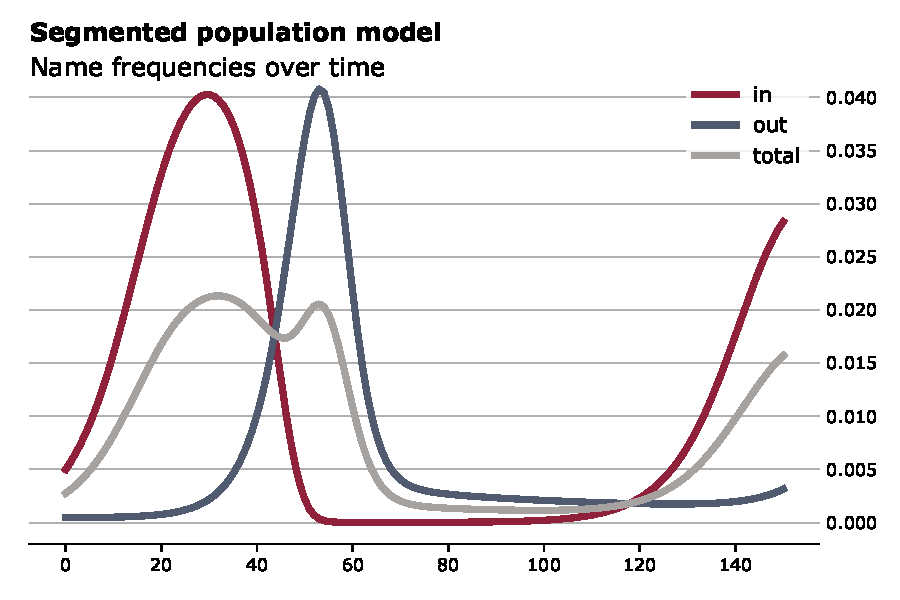
\includegraphics[width=0.9\textwidth]{figs/segmented-model.pdf}
\caption{Segmented model simulation}
\label{fig:segmented-model}
\end{figure}

In order to better understand the behavior these equations impose, we can
simulate the evolution of the in-group, the out-group, and the total popularity
of a name over time for the evolution of the model, for instance we depict one
such configuration in \cref{fig:segmented-model}. In it, we have assumed that
the in-group and the out-group are equally represented (each constitutes 50\% of
the total population), but this need not be the case. If we make the out-group
be the majority of the population, we simply get that the popularity of the name
in the entire population very closely follows the popularity of the name in the
out-group.

\begin{figure}[h]
\centering
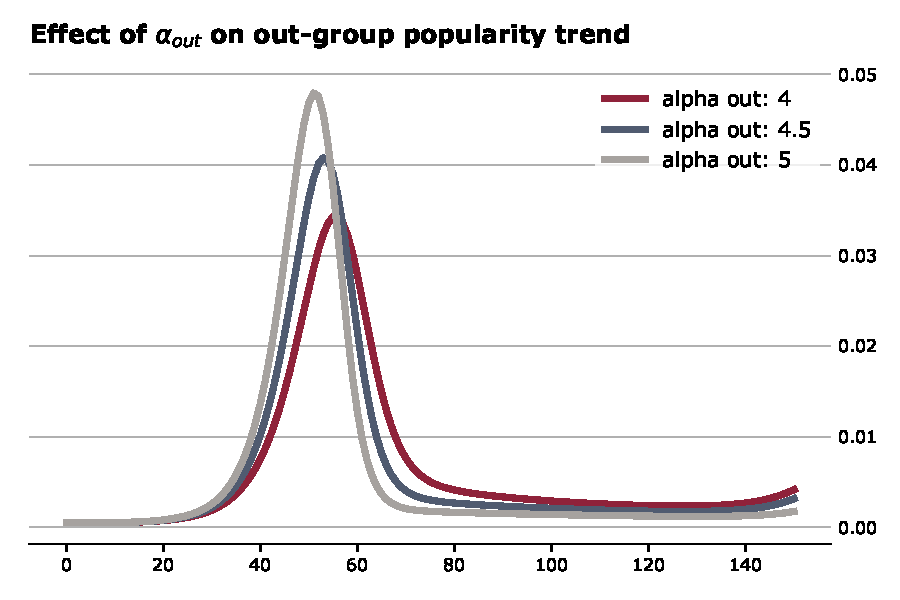
\includegraphics[width=.9\textwidth]{figs/alpha-out.pdf}
\caption{Effect of $\alpha_\text{out}$ on popularity trend}
\label{fig:alpha-out}
\end{figure}

Given our ability to numerically simulate, we can then understand the effect of
different parameters by varying them and seeing how they affect the curve. For
instance, consider the parameter $\alpha_\text{out}$ which measures the
sensitivity to incentives in the out-group. The bigger it is, the faster
out-group members move toward desirable names and away from undesirable names.
We would thus expect bigger values of $\alpha_\text{out}$ to correspond to faster
boom-bust life-cycles, as well as to higher absolute levels of popularity
(because the lag is held constant, a fast response to incentives means a bigger
increase in the name popularity before it starts going down. Both of these
predictions hold in the data, which we can see in \cref{fig:alpha-out}.

\begin{figure}[h]
\centering
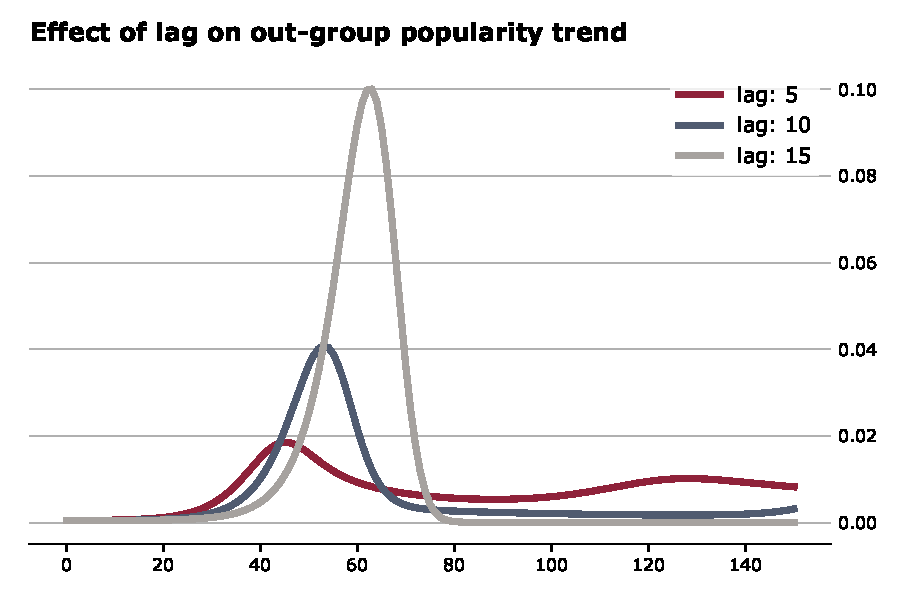
\includegraphics[width=.9\textwidth]{figs/out-lag}
\caption{Effect of lag $\tau$ on popularity trend}
\label{fig:out-lag}
\end{figure}

We expect the lag in our model to have similar effects on the maximum popularity
of a name: the longer the lag, the more popular the name will become because the
out-group continues adopting the name for a longer time before realizing it is
no longer desirable. However, we expect an opposite effect on the boom-bust
lifecycle duration: a longer lag will lead to a longer duration of the adoption
period. These conclusions are confirmed in \cref{fig:out-lag}.

Thus, when we fit the model to an observed name's popularity trend we are able
to match the empirical trend with a theoretical one by fitting these parameters
to the shape of the curve. Most notably, the attributes of the curve that are
matched include,

\begin{itemize}
\item The maximum height of popularity.
\item The duration of the up-swing
\item The duration of the down-swing
\item Whether the curve has two peaks
\end{itemize}

\subsection{Fitting the model}

Thus far we have explored the effect of different parameters on the model
output, gaining an intuition for how the model behaves. However, if we wish to
use this model for prediction we need to be able to fit to data. To do this, we
use an optimization library (\texttt{scipy}) to minimize our squared error loss
using the Nelder-Mead optimization procedure on all parameters except the lag,
which because it must be an integer is trained through a grid-search instead.

We find numerical instability for random initialization of our parameter vector.
This is a complication to batch training, and we discuss it more in the
evaluation of our model. However, when we initialize to hand-tuned parameters,
the optimization routine converges to locally optimal parameters, matching the
data reasonably well. For instance, we display the empirical trend for the
popularity of ``Amanda'' superimposed with the model fit in
\cref{fig:amanda-segmented}.

Parameters vary significantly across fitting the trends of different names,
which is consistent with there being significant heterogeneity in trends across
names. For ``Amanda'' our optimal fit tells us that the proportion of the
in-group is approximately $25\%$, the $\alpha$s are between 1 and 2, the lag
comes out as 3 years, and the $\beta$ come out as approximately 6.

\begin{figure}[h]
\centering
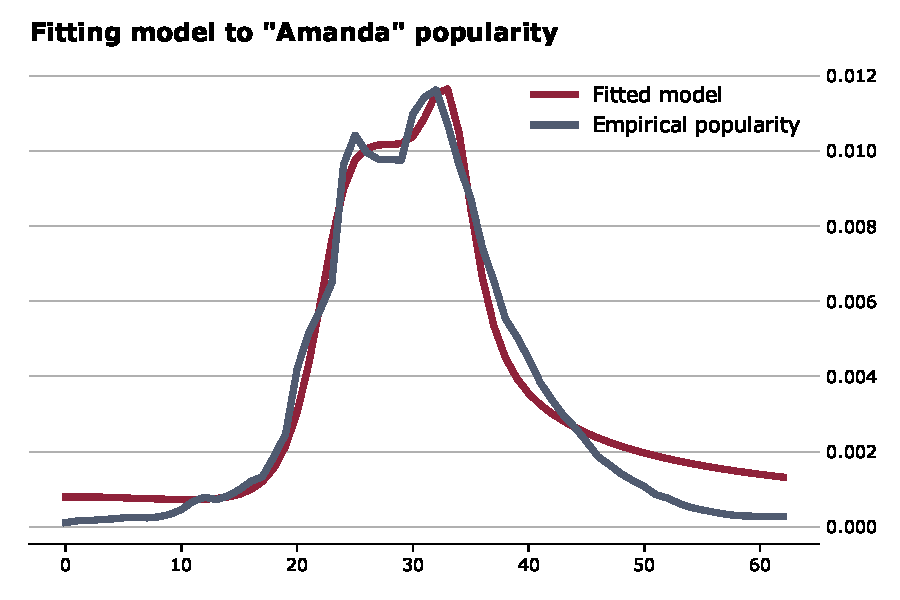
\includegraphics[width=.9\textwidth]{figs/amanda-fit.pdf}
\caption{Fit of model to ``Amanda'' trend}
\label{fig:amanda-segmented}
\end{figure}

\section{Evaluating the model}

The model has a number of strengths. At the forefront of these strengths is the
interpretability of the model underpinnings. The agents in the model (members of
the in-group and out-group) behave in an intuitively appealing way. That is, the
model sheds light on what we believe the underlying behavior is being driven by. 

In addition, the model has the flexibility to match the data we observe. Unlike
the simple imitation model which under-predicts the variance, this model can
closely track the wide variety of trends that we observe in the data. The
parameters of the model are also interpretable, since we can reason about their
effects intuitively as well as through numerical simulation.

Finally, the model makes predictions about the data that are confirmed. For
instance, the model suggests that trends should have one or two peaks depending
on the proportion of the in-group, and this is empirically confirmed.

However, the model also has some significant weaknesses. Foremost among these is
the number of parameters that need to be estimated. The large number of
parameters make us wary of overfitting. Even though the parameters are
interpretable, they are not directly observable, which also makes the fitting
process complicated. From our work, we see that the fitting process is sensitive
to initial conditions, which complicates the use of our model for a generic
trend. 

At a higher level, there are also important limitations to what our model
captures. Perhaps most relevantly, the model has no underlying theory to why
different names should have different trends / parameters. A more complete
model would have to answer the different question of why different names behave
differently. 

\section{Future work}

One shortcoming previously noted was the large number of parameters in the
model, which decrease parsimony, lead to over-fitting concerns, and complicate
the fitting process. One way to improve the model would be to capture the same
qualitative behavior with fewer distinct parameters. One way we attempted to do
this was by setting the $\alpha, \beta$ parameters for the in and out-groups to
be the same.  Unfortunately, that constraint led to oscillatory behavior
counterfactual to observed trends. Nevertheless, we believe it should be
possible with a smart constraint to simplify the parameter space while
maintaining the model's ability to capture the data.

A strength we tout is the interpretability of model's the underlying generation
process. However, future work is needed to determine whether this generation
process is actually indicative of reality. In particular, our model hypothesizes
the existence of in- and out-groups with in-group booms preceding out-group
booms in a name's popularity. It would be reasonable to hypothesize that members
of the in-group are more famous / rich / ``elite'' than out-group members. Thus,
a testable prediction of the model is that trends among these ``elites'' should
lead country-wide popularity trends. Finding data on naming trends among these
demographics would be a pivotal test for our model.

Finally, we return to an initial ambition of the project, which was to also
model the spatial component of name popularity. In this work, we have modeled
the temporal aspect by looking at name popularity over time. It would be
interesting to take the generative model we have posited and adapt it to also
make predictions about how name popularity will diffuse geographically.




\bibliography{sources}
\bibliographystyle{apalike}

\end{document}


